\begin{block}{Neural Network Training and Performance}

To train the neural networks, we add noise to the data using their respective covariance matrices. We obtain very accurate results from both approaches, with the full-shape model performing considerably better.\\

    \begin{figure}[h]
        \centering
        \begin{subfigure}{0.42\textwidth}
            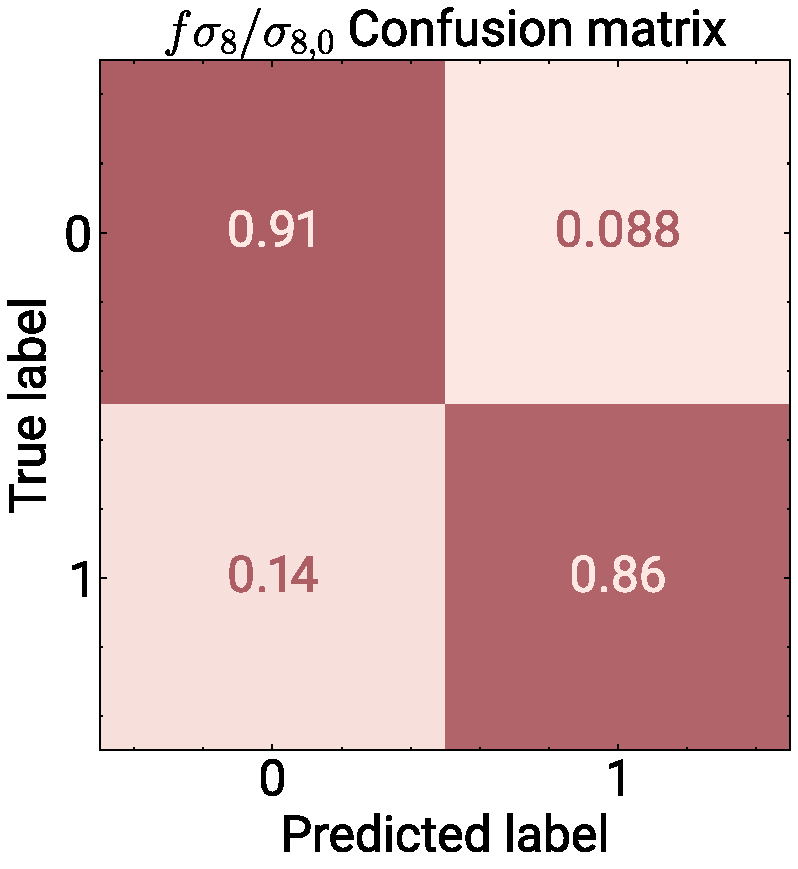
\includegraphics[width=\textwidth]{figures/fs8_cm.pdf}
        \end{subfigure}\hfill
        \begin{subfigure}{0.42\textwidth}
            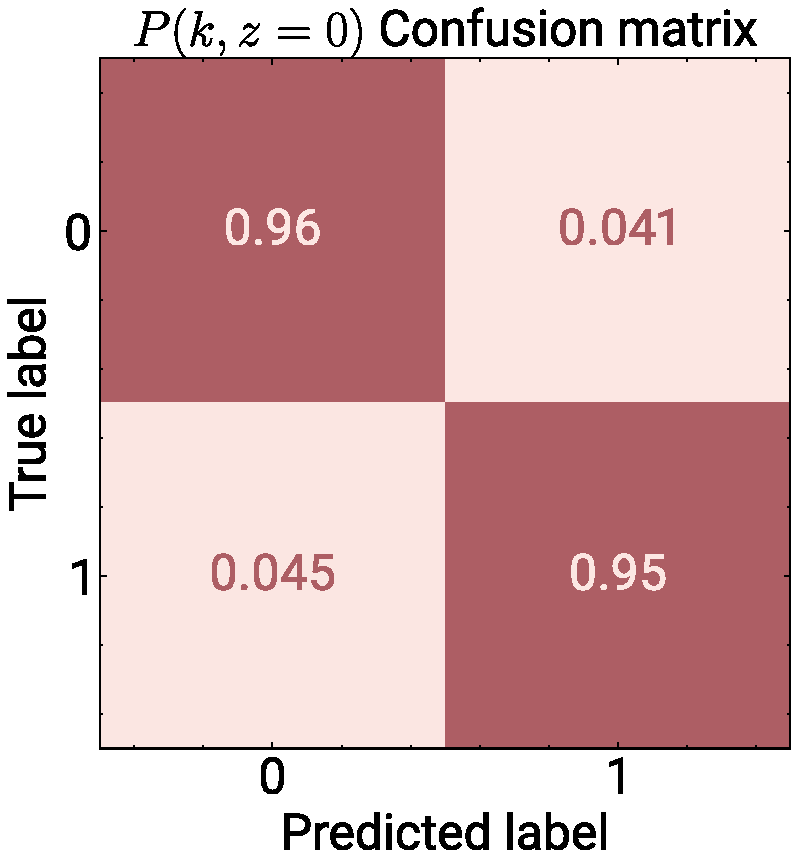
\includegraphics[width=\textwidth]{figures/Pk_cm.pdf}
        \end{subfigure}
        \caption{Confusion matrix for both models, where 0 is the label for \lcdm and 1 for HS.}
    \end{figure}
\vspace{3ex}
\end{block}
 
